\chapter{Introdução}
\label{cap:1intro}
\pagenumbering{arabic}

Um aspecto importante nas ciências físicas é poder inferir sobre parâmetros
físicos a partir de dados. Em geral, as leis da física disponibilizam os
artefatos necessários para calcular valores de dados, a partir de um modelo.
Este procedimento é conhecido como problema direto (\textit{forward problem}).
A modelagem direta, portanto, inicia com um modelo, sobre o qual um experimento ou processo
é simulado matematicamente. Se o modelo estiver correto, a resposta
obtida deve parecer com dados reais. O processo de inversão faz exatamente o contrário,
consiste em utilizar as medidas efetuadas para inferir os valores de parâmetros que
caracterizam o sistema \citep{tarantola}. Muitas vezes, o problema inverso se caracteriza
por ser não determinístico.

Considere o seguinte exemplo: imagine um exame de eletrocardiograma (ECG). Neste exame,
a corrente elétrica responsável pelos batimentos cardíacos
pode ser medida  através da disposição de eletrodos sobre a superfície do corpo,
próximos e distantes do coração. Partindo da suposição de que um coração doente
seja examinado, é possível para a um médico identificar no ECG os padrões que ratificam
a existência de um problema (problema direto). Neste contexto, o objetivo do problema inverso
é recuperar a atividade elétrica e fisiológica do coração dado um conjunto de dados de ECG.
Como a maioria dos problemas inversos, o problema inverso do exame de ECG recai sobre duas características
comuns. Primeiro, a não unicidade de solução, ou seja, o mesmo conjunto de medidas
observadas no exame pode resultar de mais de uma configuração do coração doente. Segundo,
a natureza mal-posta do problema inverso, isto é, uma pequena mudança arbitrária nos
valores observados no ECG pode causar uma mudança grande da solução fonte equivalente.

\section{Problema Inverso}

A teoria de inversão é utilizada em diversas áreas para inferir os valores de
parâmetros relacionados com processos importantes a partir dos dados medidos,
também chamados de dados experimentais. Pode-se descrever o problema inverso
como o processo de obter informações de um sistema parametrizado, a partir de
dados observáveis, das relações teóricas dos observáveis com os parâmetros não
observáveis e do conhecimento \textit{a priori} sobre os não observáveis.

O procedimento científico para o estudo de um sistema físico pode ser dividido
em três passos: a parametrização do sistema, a  modelagem direta e a modelagem inversa.
O problema da modelagem inversa, por sua vez, se caracteriza pelo
uso de resultados atuais das medições dos parâmetros físicos observáveis, para inferir os valores atuais dos
parâmetros do modelo. A maioria dos problemas inversos podem ser escritos em uma forma discreta como:
\begin{equation}
\label{eq:deqgm}
F(m) \approx d 
\end{equation}
onde, $m=(m_1, m_2,...,m_n) \subset R^n$ é o modelo estimado que pertence a um conjunto de modelos $M$ admissíveis
em termos de conhecimento prévio (\textit{à priori}). O termo $d \in R^s$, são os dados observados e
\begin{equation}F(m)=(f_1(m),f_2(m),...,f_s(m))\end{equation} representa o direto.

Na prática $d$ pode ser uma função no domínio do tempo e/ou espaço, ou pode ser
uma coleção de observações discretas. Uma questão relevante é a presença de
ruído nas observações. Geralmente considera-se que os dados são observações
de um experimento perfeito $d_v$ mais uma componente de ruído $e$:
\begin{equation}
\begin{split}
d &= F(m_v) + e \\
&= d_v + e
\end{split}
\end{equation}
onde $d_v$ satisfaz  \ref{eq:deqgm} para o modelo considerado verdade $m_v$, 
$d_v = G(m_v)$, assumindo o operador $G$ como exato. Em muitos casos é possível
ajustar matematicamente todas as partes do ruído $e$ utilizado a equação \ref{eq:deqgm},
deixando o ruído aparecer no modelo encontrado. Situação que na prática é
indesejável, pois em muitos casos uma solução de $m$ que é influenciada por até
mesmo um pequeno ruído $e$ pode ter pouca similaridade com o modelo verdadeiro
$m_v$ \citep[p. 19]{aster2013parameter}.

\section{Inversão Sísmica}

No contexto da indústria de óleo e gás, o problema de inversão sísmica é
importante para o processo de caracterização de reservatórios de
hidrocarbonetos, que consiste na determinação tridimensional e quantitativa da
estrutura e das propriedades petrofísicas (porosidade, densidade, etc) das
rochas da subsuperfície. O método de aquisição sísmica de reflexão utiliza
pulsos sísmicos de uma fonte artificial controlada e monitora a resposta em
função do tempo. Neste sistema, cada interface entre dois tipos de rochas
diferentes gera reflexão e refração do pulso sísmico, como demonstrado na Figura
\ref{fig:1sismica}.

\begin{figure}[ht!]
\begin{center}
  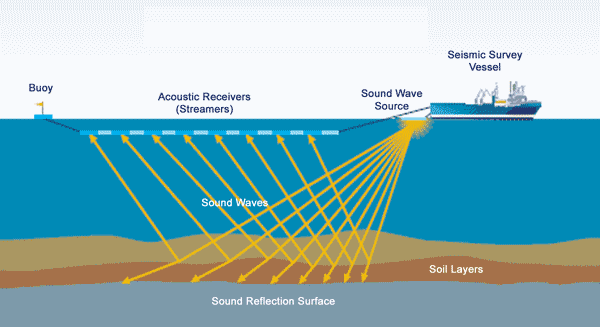
\includegraphics[width=0.8\textwidth]{fig/seismic_survey}
  \caption{Método de sísmica de reflexão \citep{figsismica}}
  \label{fig:1sismica}
\end{center}
\end{figure}


Para inversão acústica, o modelo mais utilizado para representar a resposta do
pulso sísmico atravessando as interfaces entre rochas é o convolucional. Nele é
assumido um modelo em camadas para a subsuperfície e ângulo de incidência e
reflexão de $90^\circ$. A medida efetuada é representada pelo resultado da
convolução do pulso sísmico, também chamado de \textit{wavelet}, com as
refletividades das interfaces. Os coeficientes de reflexão com ângulo de
reflexão normal são modelados por \citep[p. 69]{sen_livro}:

\begin{equation}
r(t) = \frac{z(t+\delta t)-z(t)}{z(t+\delta t)+z(t)}
\end{equation}
onde $z(t)$ é a impedância acústica no tempo $t$ definida por
$z(t)=\rho(t)v(t)$, onde $\rho(t)$ é a densidade da rocha e $v(t)$ a
velocidade de propagação da onda acústica. Utilizando os coeficientes de
reflexão, modela-se a resposta do sistema $d(t)$ aplicando a convolução
da \textit{wavelet} $s$ com os coeficientes de refletividade:

\begin{equation}
d(t) = \int_{-\infty}^{\infty} s(\tau)r(t-\tau)d\tau + e_d(t)
\end{equation}
onde é assumida a presença de um ruído aleatório $e_d(t)$ e $d$ é o chamado dado
sísmico. Cada sequência de dados $d$ representa um ponto no plano $xy$ e suas
posições $(t)$ são coordenadas em tempo que se relacionam com a profundidade.
Cada $d_{xy}$ é muitas vezes chamado de traço sísmico, o que no caso discreto
pode ser uma coluna de uma matriz 2D, por exemplo. Um conjunto de traços
sísmicos também é chamado de uma imagem, seção ou cubo, no caso de um
levantamento 3D. A \textit{wavelet} ideal seria um pulso tipo delta contendo
todas as frequências, mas gerar tal pulso não é viável. Na prática as
\textit{wavelets} são pulsos de banda limitada entre $6Hz$ e $65Hz$, o que
limita a frequência da sísmica e sua resolução \citep[p. 11]{sen_livro}.
A Figura \ref{fig:wavelet} ilustra uma \textit{wavelet} típica extraída de dados
reais.

\begin{figure}[htp]
\begin{center}
  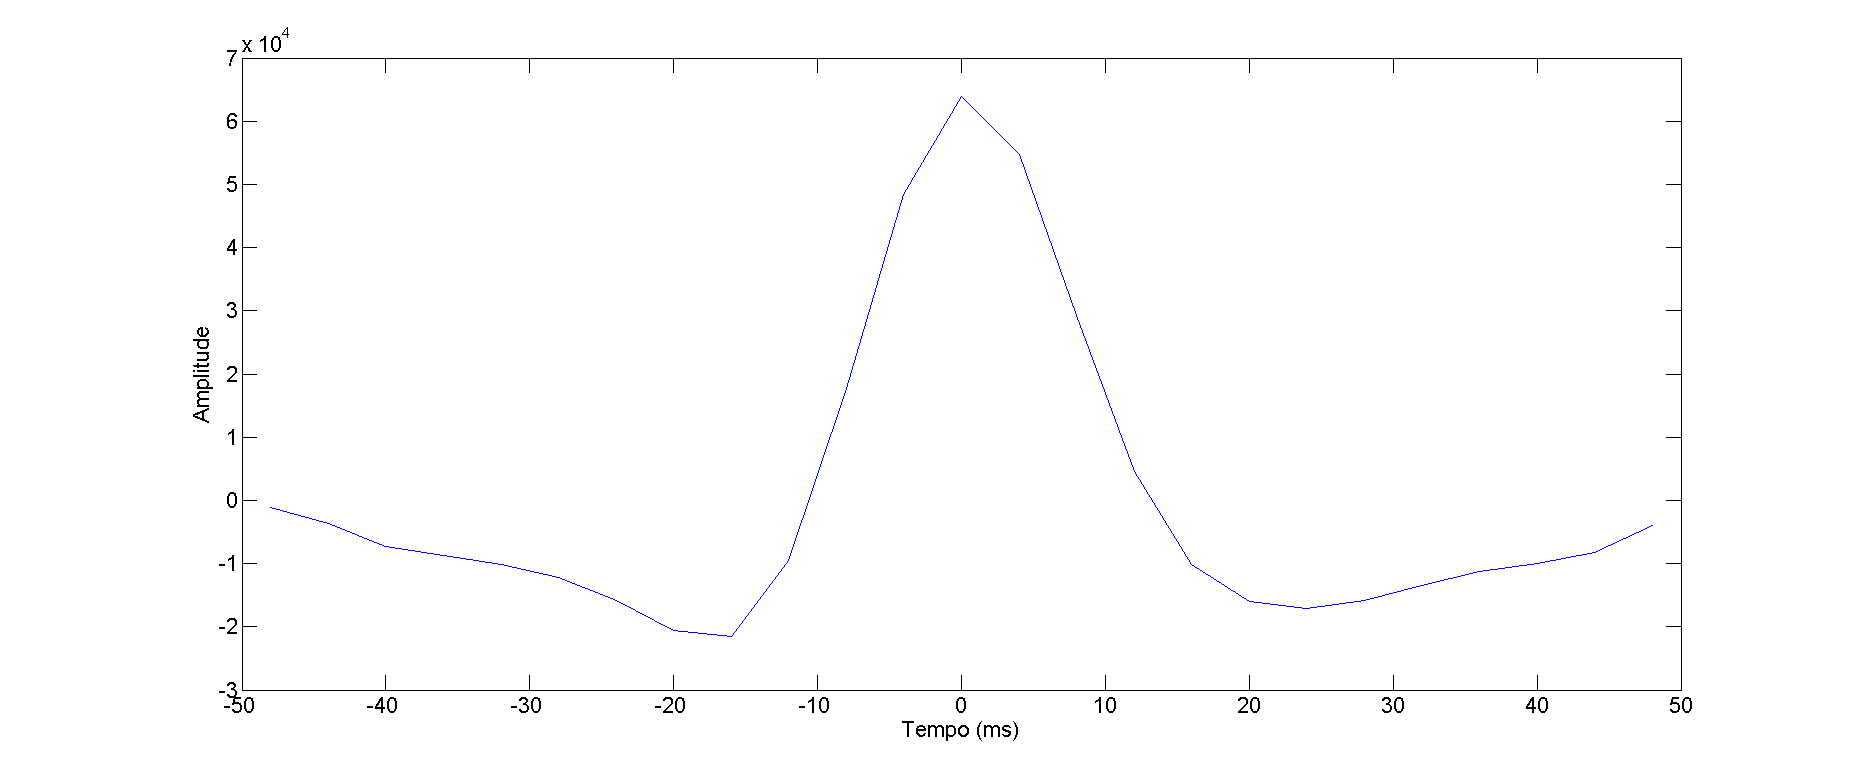
\includegraphics[width=0.8\textwidth]{fig/wavelet}
  \caption{\textit{Wavelet} extraída de dados reais}
  \label{fig:wavelet}
\end{center}
\end{figure}

O objetivo da inversão sísmica acústica é determinar os valores de impedância
acústica das camadas de rocha. Esse é um problema não linear, pois as equações
que determinam o modelo direto são não lineares. Também é considerado mal posto,
pois é ambíguo, ou seja, várias combinações de camadas e suas impedâncias podem
gerar o mesmo resultado no dado sísmico. Essas características geram a
necessidade de alta intervenção de especialistas para restringir o resultado
(regularização). Quando poços são perfurados, são utilizadas outras ferramentas
para observar dados mais próximos aos reais. Os principais métodos de inversão
utilizam os dados de poços para regularização e geração de estatísticas.

No processo de inversão é importante a modelagem da incerteza dos resultados
obtidos, ou seja, obter soluções equivalentes respeitando os dados medidos e as
informações \textit{a priori}. Essas soluções devem representar bem a região
onde o erro é menor que a tolerância desejada, chamada de região de equivalência
\citep{tompkins_comparisonBayes}. Existem várias razões para essa região de
equivalência existir, incluindo erros nas medidas, cobertura dos dados sobre a
as localizações desejadas, limitação de banda do pulso sísmico, suposições sobre
o modelo físico (e.g. isotropia, modelo de camadas, homogeneidade, etc.) e
aproximações matemáticas do modelo direto. A modelagem de incerteza ajuda na
avaliação dos riscos envolvidos nos processos de perfuração, exploração e
produção de óleo e gás.

As médias e variâncias locais das soluções não são suficientes para caracterizar
a incerteza na inversão, pois os modelos de impedância geralmente são utilizados
como entrada de processos como a simulação de fluxo. Esse tipo de simulação é
essencialmente uma função não linear, ou seja, a média das simulações de fluxo
não é necessariamente igual a simulação da média das impedâncias:
$F(\overline{\mathbf{m}})\neq \overline{F(\mathbf{m})}$, onde ${\mathbf{m}}$
representa as soluções aceitáveis, $F(\cdot)$ a função não linear da
simulação de fluxo e $ \overline{(\cdot)}$ a operação de média. Amostragem, de
uma forma geral, possibilita análises mais sofisticadas da distribuição
posterior \citep{hansenGibbsPrior}.

%TODO importancia das realizações na modelagem, ainda falta citação da
% simulacao de fluxo (funcao nao linear)

 Na literatura recente, diversos métodos foram propostos para tentar solucionar
 o problema da inversão sísmica com modelagem de incerteza.
Modelos envolvendo técnicas de inteligência computacional foram propostos para
tentar resolver o problema
\citep{senSimulatedAnnealin,MallickGeneticInve,max_inv_simulated,Artun2011143,MartinezPSO,Sambridge22102013}.
Apesar de terem oferecido bons resultados, esses modelos baseados em otimização
não capturam de forma ideal o conhecimento do especialista. A incerteza
resultante desses métodos é relacionada com o nível em que foi explorada a
superfície de erro, ao invés da incerteza relacionada aos dados e conhecimentos
\textit{a priori} inseridos.

O uso de ferramental probabilístico baseado no teorema de Bayes pode ser
aplicado, em conjunto com o amostrador de Gibbs, para gerar realizações
estocásticas da distribuição \textit{a posteriori} \citep{leandro_SEG}. Assim,
pode-se computar estatísticas do conjunto de soluções, obtido à alto custo
computacional. Para atacar a maldição da dimensionalidade e diminuir o custo da
amostragem de soluções, foram propostos métodos que utilizam redução dimensional
\citep{TompkinsScalabUnce2011}. Neste caso, aplicando análise de componentes
principais (PCA) é possível reduzir a dimensão do problema e utilizar um esquema
de amostragem determinística, ao custo de perda na resolução espacial das
amostras.

\section{Simulação Multiponto}



\section{Redes Neurais Convolucionais}
Nesta seção a convolução será descrita. Serão apresentados os principais conceitos relacionados às redes
neurais convolucionais e sua estrutura e as principais
aplicações deste modelo de aprendizagem de máquina. Um ponto não abordado nesta seção é
como escolher a arquitetura de uma rede convolucional.

As redes convolucionais, também chamadas de redes neurais convolucionais (CNN),
são um tipo de rede neural especializada em processamento de dados que possuam uma
topologia conhecida e em forma de grade. Exemplos deste tipo de dado são as séries
temporais, que podem ser vistas como uma grade em uma dimensão (1D) com amostras
em intervalos de tempo regulares, e dados de imagem, que podem ser pensados como
uma grade 2D de \textit{pixels}. As redes convolucionais são um tipo de rede neural
que usa a operação de convolução no lugar de multiplicação de matrizes em pelo menos uma
de suas camadas.

\subsection{Convolução}

A operação de convolução costuma ser denotada com um asterisco (Eq. \ref{eq:1}).
Na Equação. \ref{eq:1}, $x$ refere-se ao conjunto de imagens de entrada, uma sequência multidimensional
de dados, e $w$ é denominado \textit{kerenl} ou filtros, uma sequência multidimensional de parâmetros otimizados pelo algoritmo
de aprendizagem.
\begin{equation}
 s(t) = (x * w)(t)
 \label{eq:1}
\end{equation}

A convolução se sustenta sobre três pilares: interações esparsas, compartilhamentos
de parâmetros e representações equivalentes. As redes neurais tradicionais
utilizam a multiplicação de matriz por uma matriz de parâmetros para descrever
a interação entre cada unidade de entrada e cada unidade de saída. Isso
significa que toda unidade de saída interage com toda unidade de entrada.
As redes convolucionais, por outro lado, tipicamente possui interações
esparsas, também chamadas d conectividade esparsa ou pesos esparsos.
Para isto, é necessários que os filtros sejam menores que a entrada.
De um ponto de vista prático, no processamento de uma imagem,
a imagem de entrada pode ter milhares de pixels, entretanto, é 
possível detectar apenas pequenas regiões de características importantes,
por exemplo com significado geológico, com filtros que compreendam apenas
algumas dezenas ou centenas de pixels na imagem. Como consequência,
menos parâmetros são armazenados e aumenta a eficiência estatística do
modelo. As figuras \ref{fig:full} e \ref{fig:sparse} ilustram
os modelos citados anteriormente. É possível notar que o número de elementos
que afetam elemento de saída em destaque ($s_3$) é definido pela convolução
com filtro de largura 3 (figura \ref{fig:sparse}), por outro lado $s_3$ é
afetado por todos os elementos da entrada quando formado por multiplicação
matricial (figura \ref{fig:full}).

\begin{figure}[htp]
\begin{subfigure}{.5\textwidth}
  \centering
  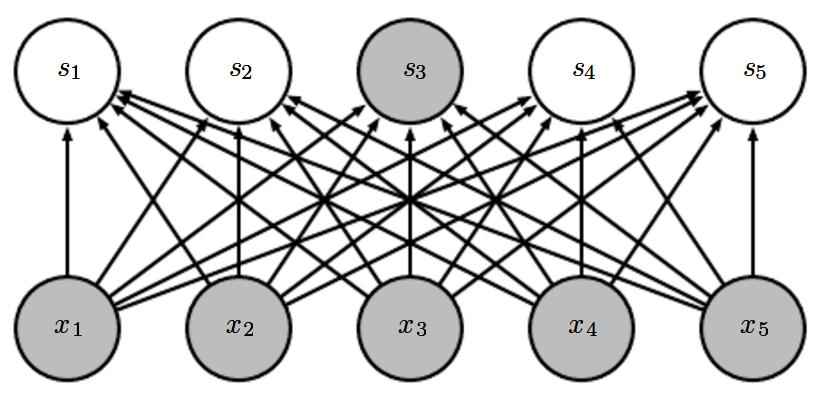
\includegraphics[width=.9\linewidth]{fig/full_conections}
  \caption{Conectividade tradicional.}
  \label{fig:full}
\end{subfigure}%
\begin{subfigure}{.5\textwidth}
  \centering
  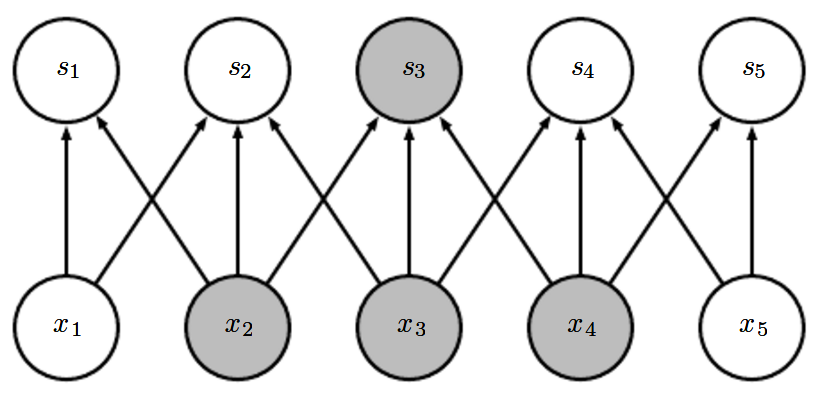
\includegraphics[width=.9\linewidth]{fig/sparse_conections}
  \caption{Conectividade esparsa.}
  \label{fig:sparse}
\end{subfigure}
\end{figure}

O \textbf{compartilhamento de parâmetros}, também chamado de \textbf{pesos amarrados} 
em uma rede convolucional se refere ao uso do mesmo parâmetro para mais de uma função no modelo.
Nas redes neurais tradicionais, cada elemento da matriz de pesos é usado apenas uma vez quando a
saída da camada é calculada, pois é multiplicado por apenas um elemento da entrada. No compartilhamento
de pesos, o valor do peso aplicado a uma entrada está relacionado ao valor de um peso aplicado em
algum outro local. Na rede convolucional, cada elemento do filtro é usado em toda posição da entrada,
de modo que, ao invés de aprender um conjunto separado de parâmetros toda localização da imagem, apenas
um conjunto é aprendido.

\subsection{Pooling}
Uma camada em uma rede convolucional consiste de três estágios. No primeiro estágio,
a camada realiza diversas convoluções para produzir um conjunto de ativações lineares.
O segundo estágio é chamado etapa de detecção, na qual cada ativação é submetida a uma
função não-linear. A terceira etapa é chamada de \textit{pooling}, responsável por
modificar a saída para o resumo estatístico das saídas em uma determinada vizinhança. A operação de
\textit{pooling} permite tornar invariante pequenas translações no conjunto de entrada,
ou seja, ainda que haja pequenas translações na entrada, os valores da maioria das saídas após a
o \textit{pooling} permanecem iguais. A figura \ref{fig:pool} ilustra o funcionamento da função de \textit{pooling}.
\begin{figure}[htp]
\begin{center}
  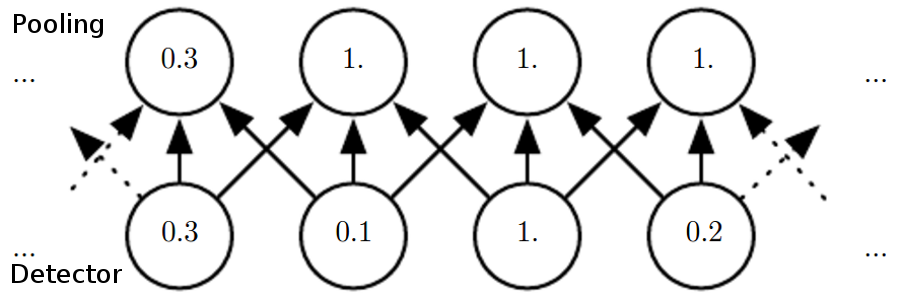
\includegraphics[width=0.7\textwidth]{fig/pool}
  \caption{Operação de \textit{pooling} com região de tamanho 3. Nesta operação é selecionado o máximo valor de ativação da etapa de detecção.}
  \label{fig:pool}
\end{center}
\end{figure}

A operação de \textit{pooling} permite lidar com entradas de tamanho variável.
Classificar imagens de tamanhos diferentes, por exemplo, pode ser realizado
variando o tamanho entre as regiões de pooling de modo que a camada de 
de classificação sempre receba o mesmo número de sumários estatísticos
independente do tamanho da imagem.

\section{Objetivo}

O objetivo do presente trabalho consiste em propor um modelo capaz de integrar a
atualização Bayesiana no processo de inversão GSI. Resultados prévios indicam
que utilizar ...

Outro objetivo é ...

\section{Organização do Texto}

Este documento está organizado da seguinte forma. Após esta breve introdução, o
Capítulo \ref{cap:2modelosInversao} apresenta o estado da arte em modelos de
inversão sísmica com modelagem de incerteza. O Capítulo \ref{cap:3modeloHibrido}
trata da proposta do projeto e resultados preliminares da integração de
atualização Bayesiana em inversão Geoestatística, a ser desenvolvido em parceria
com o CERENA - Centro de Recursos Naturais e Ambiente do Instituto Técnico da
Universidade de Lisboa, sob orientação do professor Dr. Amilcar Soares,
especialista em Geoestatística e inversão sísmica. O estágio será iniciado em
julho de 2015 e terá 12 meses de duração. Após o retorno ao Brasil, estão
planejados mais 8 meses de trabalho para finalizar a escrita da tese e defesa.

